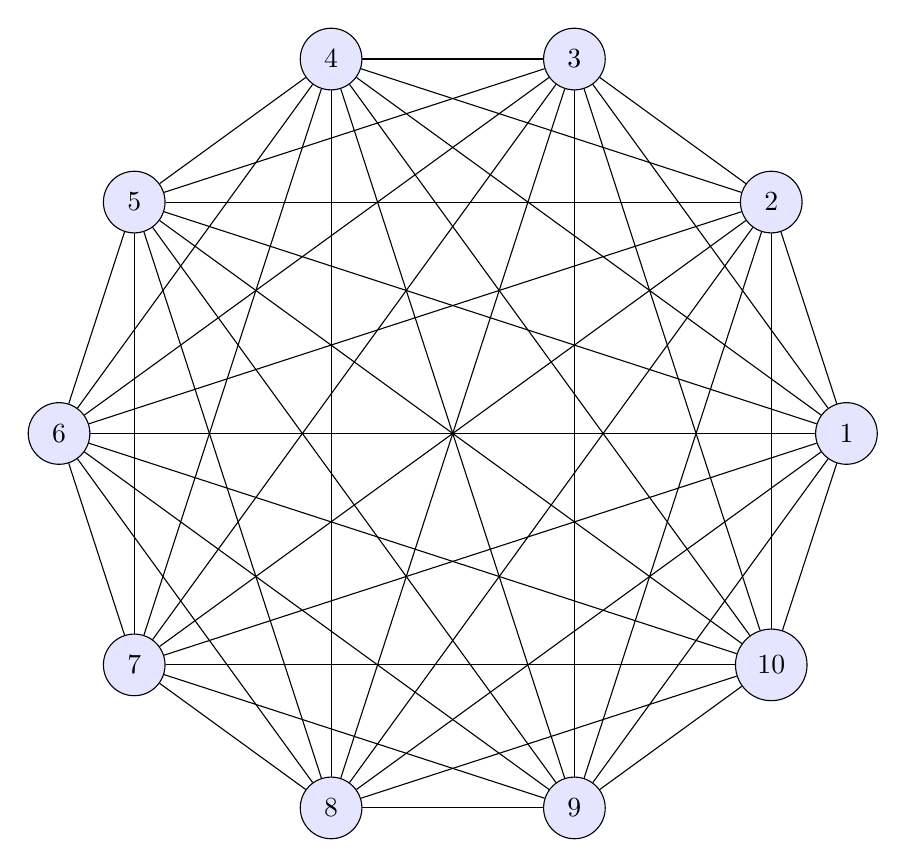
\begin{tikzpicture}

\def\nodes{10}

\foreach \x in {1,...,\nodes} {
	% Computer angle:
	
	\pgfmathparse{(\x-1)*(360/\nodes)}
	\node[draw,circle,fill=blue!10,inner sep=5] (N\x) at (\pgfmathresult:5) {\x};
}

\foreach \x [count=\xi from 1] in {2,...,\nodes} {
	\foreach \y in {\x,...,\nodes} {
		\draw (N\xi) -- (N\y);
	}
}

\end{tikzpicture}